\section{Implementation} \label{sec:implementation}
This section will discuss the implementation of each module and the way they integrate together to make the computer. Figure \ref{fig:prototypea} shows the computer as it was in February 2025. The overlays shown in Figure \ref{fig:prototypeb} show where each of the modules described in previous sections is located on the computer.

\begin{figure}[H]
  \centering
  \begin{subfigure}{0.9\linewidth}
    \centering
    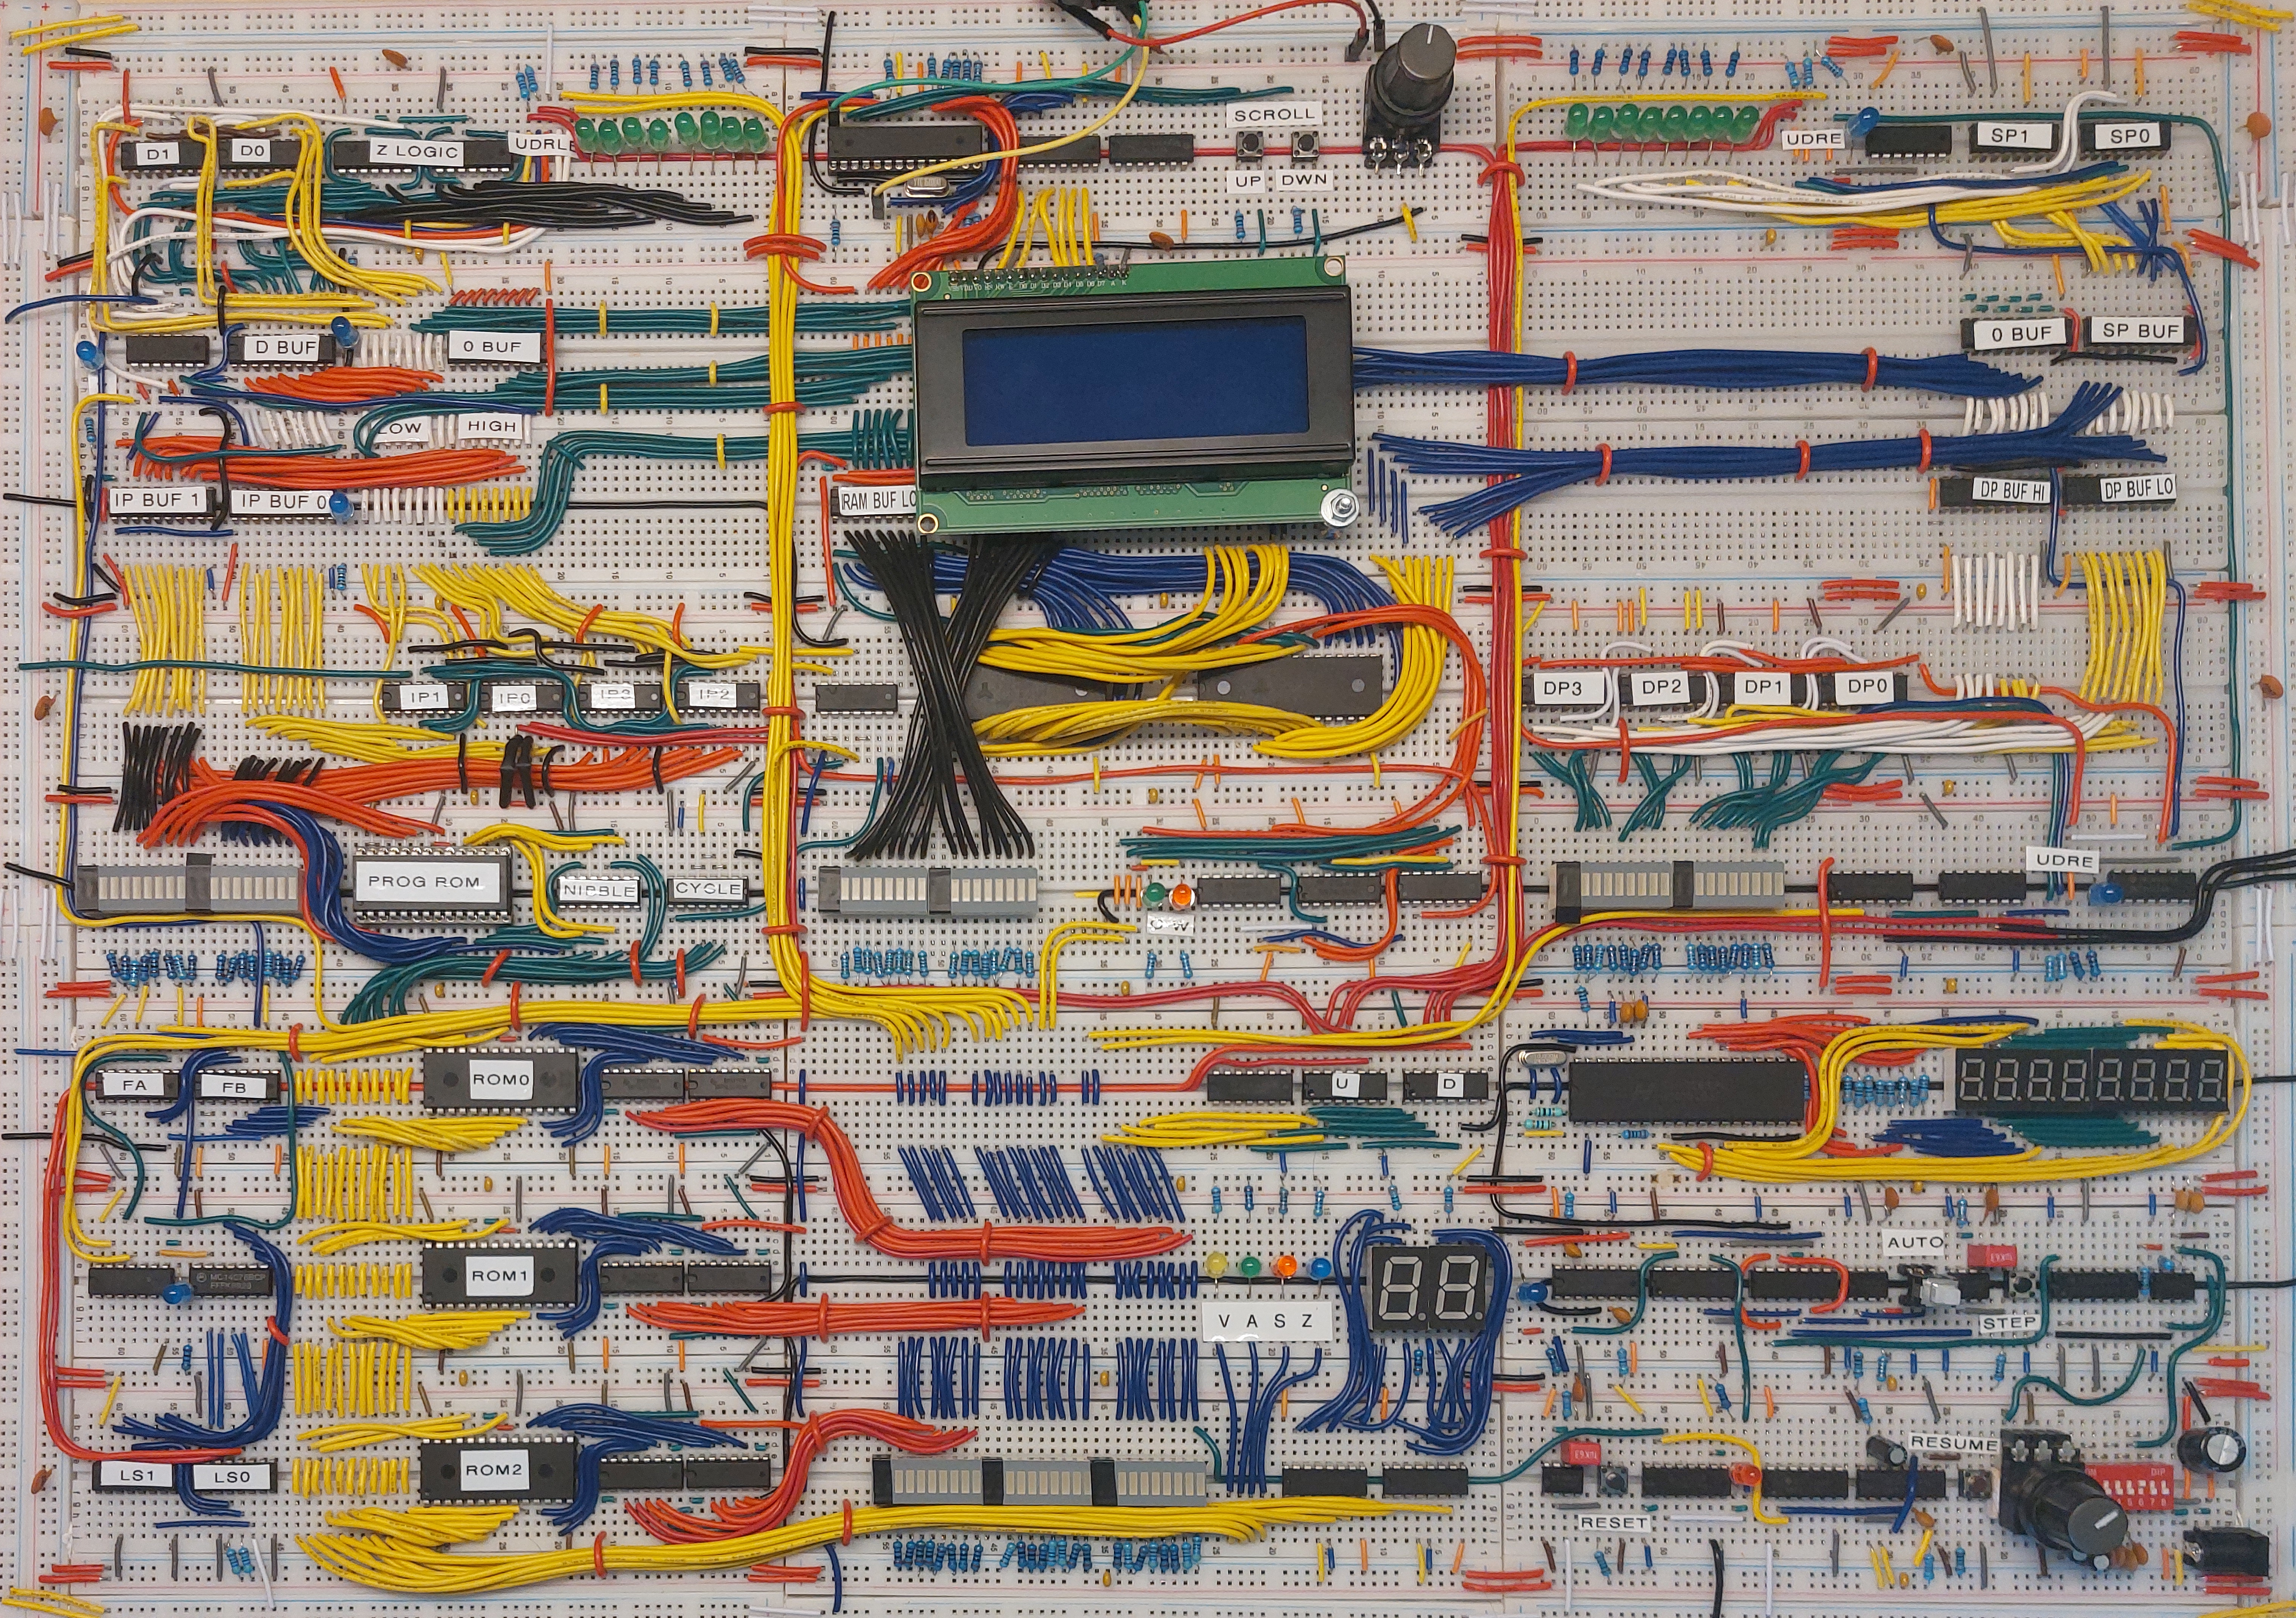
\includegraphics[width=0.8\linewidth]{img/computercloseup}
    \caption{Prototype of February 2025}
    \label{fig:prototypea}
  \end{subfigure}
  \vspace{\baselineskip}
  \begin{subfigure}{0.9\linewidth}
    \centering
    \includegraphics[width=0.8\linewidth]{img/computerparts}
    \caption{Location of the modules on the prototype}
    \label{fig:prototypeb}
  \end{subfigure}
  \caption{}
  \label{fig:prototype}
\end{figure}

%%%%%%% CLOCK

\subsection{Clock Module} \label{sec:clock}
\begin{figure}[H]
  \centering
  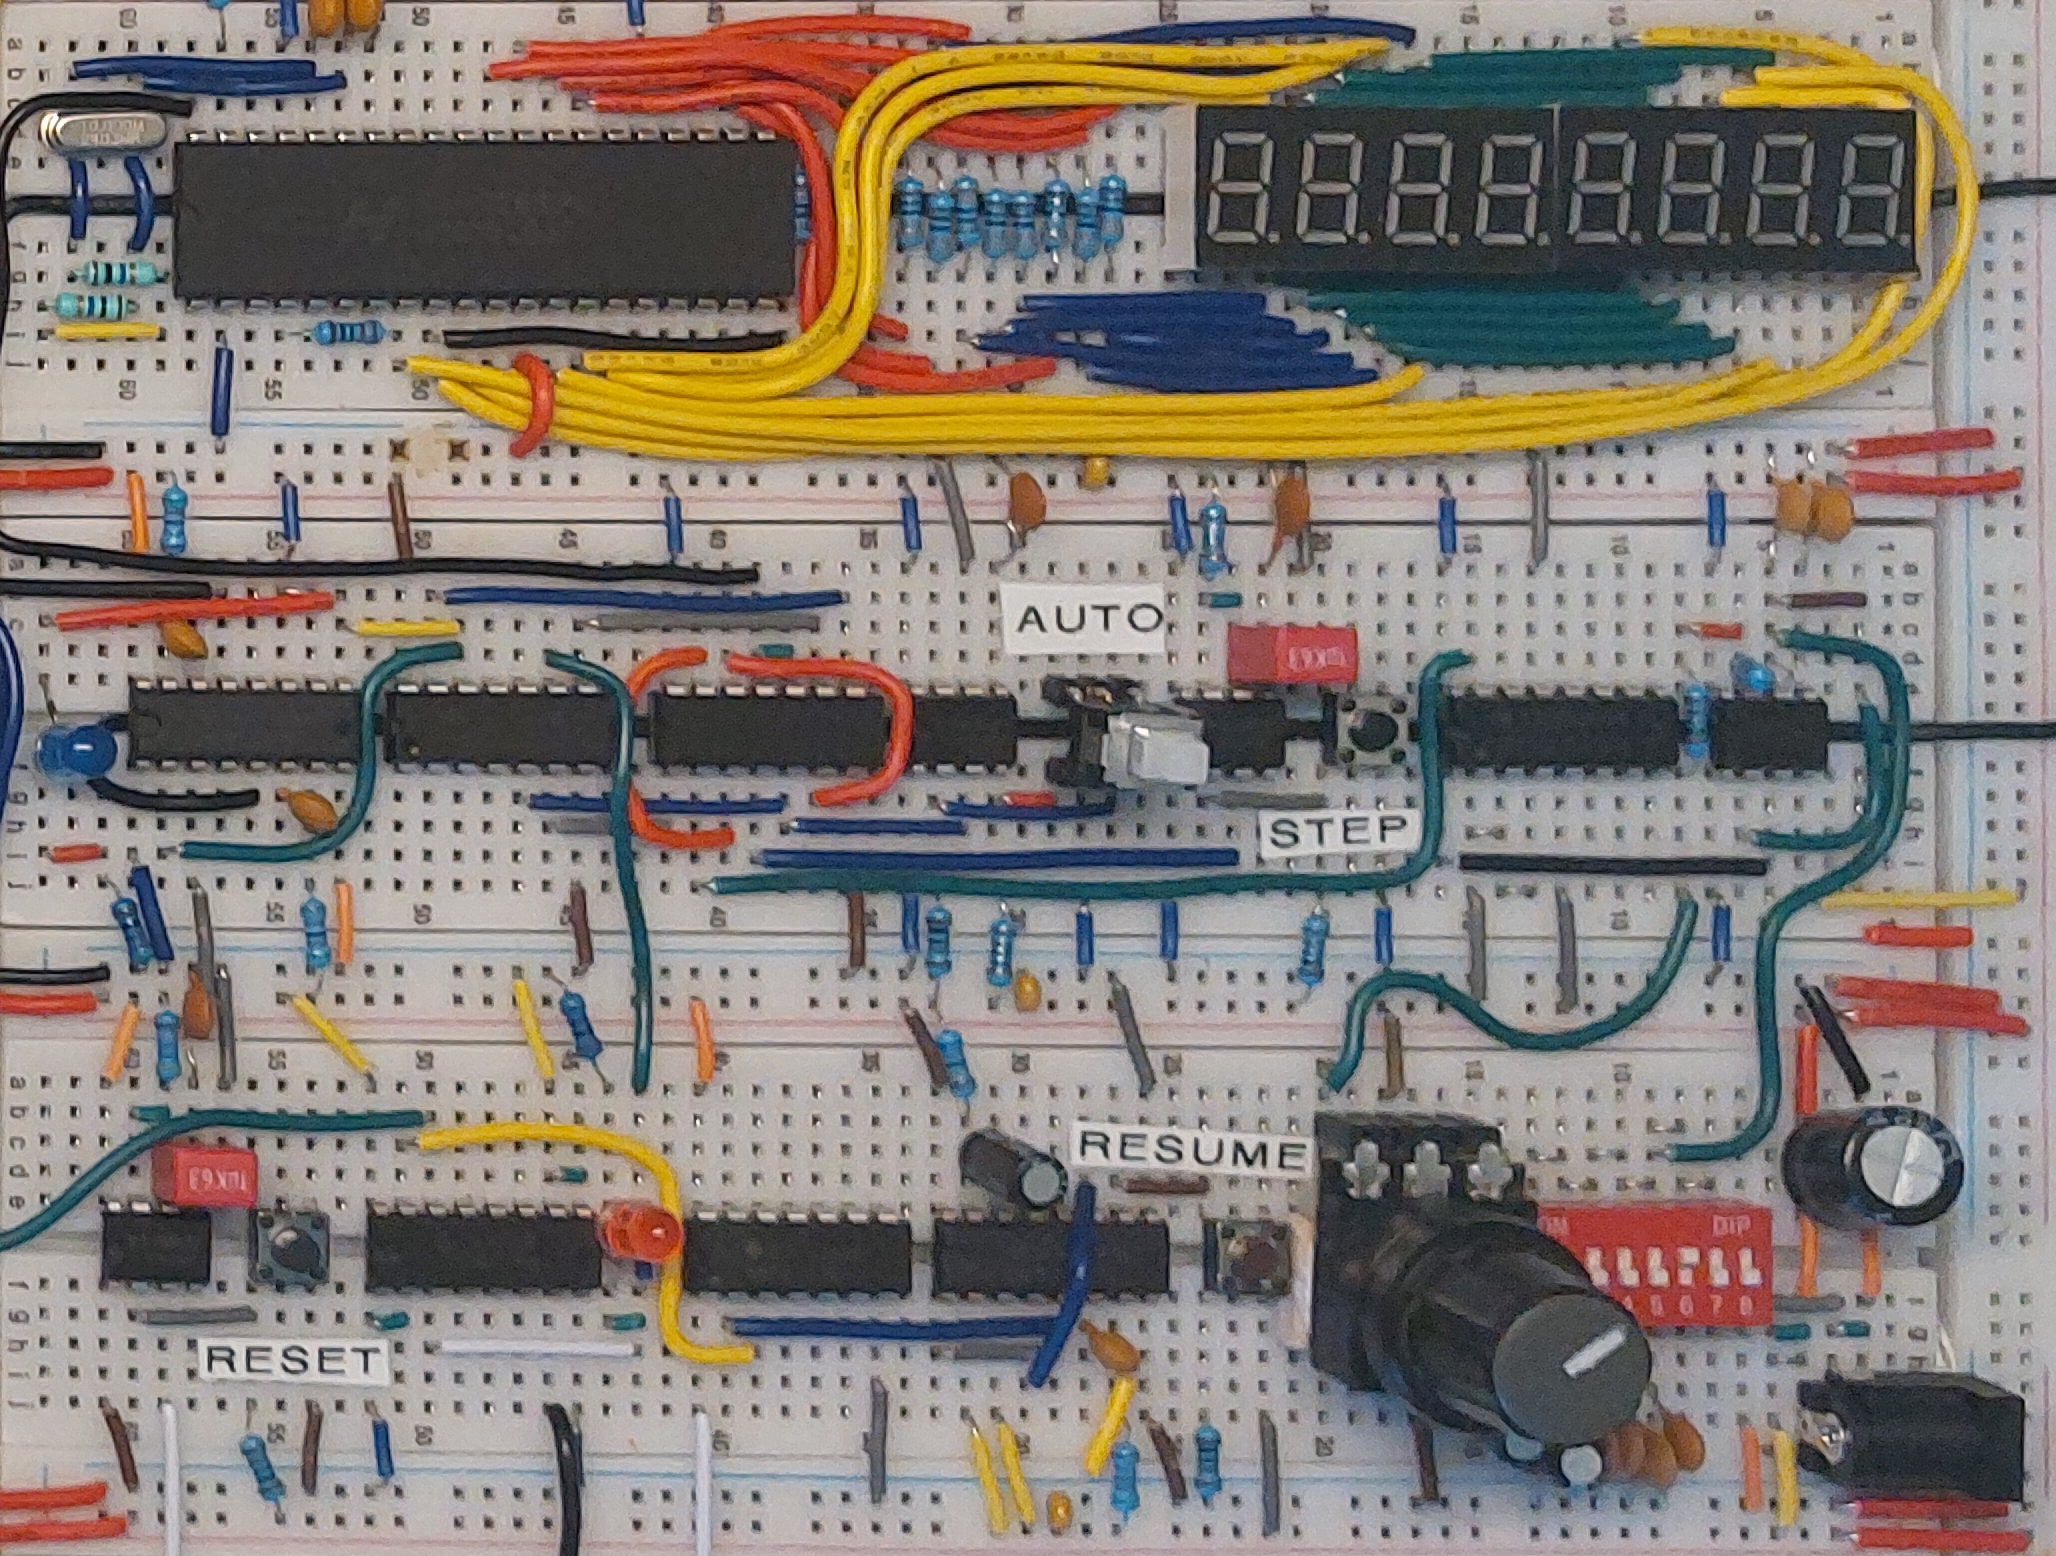
\includegraphics[width=0.6\textwidth]{img/clockmodulecloseup}
  \caption{Close up of the Master Clock and Reset/Resume Modules.}
  \label{fig:masterclockcloseup}
\end{figure}

The clock module is located at the bottom right of the computer and is responsible for providing a heartbeat to most of the modules. The design of the clock is taken directly from Ben Eater's 8-bit computer video's \cite{beneater}. The automatic clock is generated by a 555 timer in astable mode. A set of DIP switches is used to select the capacitor of the RC-circuit that determines the output frequency for coarse control and a 100K linear potentiometer is used for fine control of the clock frequency. Two additional 555 timers are used to debounce both the pushbutton for the manual clock and the latching push button which acts as a select between the two modes, as per Ben's design. 

The frequency of the astable 555 is halved by sending it through a JK flip-flop to ensure a perfectly symmetric duty cycle, then fed into divided into a 74LS123 monostable multivibrator to produce two short 200ns pulses: one on the rising and another on the falling edge the output of the flip-flop. This results in two sets of clean signals at constant intervals. On the first pulse (rising edge of the original clock), the control signals are loaded from the microcode EEPROMs into their registers (which connected to the modules), while the second pulse is connected to the modules to act upon. This approach guarantees a clean division between setting the control signals and clocking the modules. Figure \ref{fig:clocktiming} shows the timing diagram for the different signals discussed above.

\begin{figure}[H]
  \centering
  \includegraphics[width=0.6\textwidth]{img/clocktiming}
  \caption{Timing diagram for the clock signals.}
  \label{fig:clocktiming}
\end{figure}

\subsubsection{Frequency Control}
The frequency of the master clock can be set using dip switches to select the capacitor-value and a 10K potentiometer to select the resistance of the RC circuit connected to the 555 timer. The capacitor, in conjunction with a fixed 2K resistor, sets a broad range (lower capacitance corresponding to higher frequencies) while the potentiometer is used finegrained selection of the frequency within this range. This potentiometer is wired in series with a 1K resistor to enure stability when the potentiometer resistance drops toward zero. Table \ref{tab:frequencycontrol} should the frequency-ranges available for each of the currently selected capacitors. These values have been measured \emph{after} the flip-flop (so the actual frequency of the 555 timer is around double the frequencies displayed in table \ref{tab:frequencycontrol}).

\begin{table}
  \centering
  \begin{tabular}{c|r|r}
    Capacitance (F) & $f_{min}$ (Hz) & $f_{max}$ (Hz) \\ \hline
    $10^{-5}$  & 5 & 15 \\
    $10^{-6}$  & 40 & 140 \\
    $10^{-7}$  & 500 & 1,500 \\
    $10^{-8}$  & 5,000 & 14,000 \\
    $10^{-9}$  & 19,000 & 55,000 \\
    $10^{-10}$ & 38,000 & 108,000  
  \end{tabular}
  \caption{Frequency ranges for each of the capacitors (approximate).}
  \label{tab:frequencycontrol}
\end{table}

\subsubsection{Frequency Display}
To be able to see the frequency at which the computer is running, the module clock signal is connected to an ICM7226B \cite{?}, which is configured as an 8-digit frequency timer. It drives two 4-digit 7-segment displays at a 1 second interval (the frequency is measured and updated every second). For this module, no schematics will be provided.

\subsection{Reset/Resume} \label{sec:resetresume}
The Reset/Resume module is located directly underneath the clock and contains logic necessary to be able to reset the computer (necessary after applying power) and resuming the clock after it has been halted. The HLT signal coming from the decoder is latched into a register (74LS173) from which the corresponding output bit is connected to the HLT input of the clock module. When the system is reset (using the reset button) or when the resume button is pressed, the HLT bit is cleared and the clock resumes. This allows for pausing and resuming the computer, effectively adding breakpoints in the code. The reset button itself is debounced in the same way as the manual clock button to ensure a stable transition with a debounce time of around 300ms.

The Resume button needs more sophisticated debounce circuitry due to the following scenario: when multiple HLT instructions are seperated by a relatively small amount of other instructions, a pulse in the order of milliseconds (like the reset and pulse debouncers) will be far too long at high clock frequencies. The resume-signal will still be high when a second (or third, fourth, ...) HLT instruction is encountered, causing control flow to simply skip over these instructions. To remedy this situation, a debouncing circuit is required that first produces a pulse of equal width of the clock pulses (Figure \ref{fig:clocktiming}), followed by a guaranteed period where the signal is low, even when the button bounces after the pulse. This is achieved by creating a feedback loop between the two monostable vibrators present on the 74LS123. The first one will produce a 200ns pulse on the rising edge of the button. This pulse is sent to the reset of the register that holds the HLT signal in order to clear it, but is also connected to the second monostable vibrator. When the initial (short) pulse goes low, the second vibrator generates a much longer pulse that is connected to the reset-input of the first one, making sure it cannot be re-activated for some time. By selecting a 680K resistor and a 4.7$\mu F$ capacitor, a cooldown period of around a second is achieved. Figure \ref{fig:resumedebounce} shows a timing diagram to illustrate this process in more detail. 

\begin{figure}[H]
  \centering
  \includegraphics[width=0.6\textwidth]{img/resumedebounce}
  \caption{Timing diagram for the resume debouncer. The output of Monostable 1 is connected to the reset of the register that stores the HLT signal.}
  \label{fig:resumedebounce}
\end{figure}


\subsubsection{Schematic}
A full schematic is provided on the next page.
\includepdf[landscape=true]{schematics/masterclock.pdf}

%%%%%%% REGISTER DRIVER

\subsection{Register Driver} \label{sec:implementation:registerdriver}
\begin{figure}[H]
  \centering
  \includegraphics[width=0.6\textwidth]{img/registerdrivercloseup}
  \caption{Close up of the Register Driver Module.}
  \label{fig:registerdrivercloseup}
\end{figure}
The register driver is responsible for sending the correct signals to the counting input of the D, DP, SP, IP and LS registers. All of these are based around the 74LS193, which has a U and D input and requires one of them to be pulsed low in order to execute the corresponding action. For example, to decrement this register, a low pulse must be sent to the D input while U is kept high. As explained in section \ref{sec:architecture:controlunit}, we used a centralized driver to limit the number of logic IC's necessary to drive the registers and the total number of control signals necessary.

The driver module makes use of a pair of 74LS138 decoders. This chip takes 3 bits (A, B and C, connected to the register-select signals RS0, RS1 and RS2) to address one of its outputs and two gating inputs G1 and G2. When both gates are active, a low signal will be provided on the output pin determined by the address set on A, B and C. By letting the module-clock (M\_CLK) pulse one of the gates, a low pulse is created on the output selected by the values present at A, B, and C and routed to the corresponding counting module. We use the first '138 for generating the U signal and the second '138 for the D signal. The INC and DEC signals are connected to the other gates to determine which of the decoders is generating the pulse.

\subsubsection{Schematic}
A full schematic is provided on the next page.
\includepdf[landscape=true]{schematics/registerdriver.pdf}

%%%%%%% DATA POINTER REGISTER

\subsection{DP Register Module}
\begin{figure}[H]
  \centering
  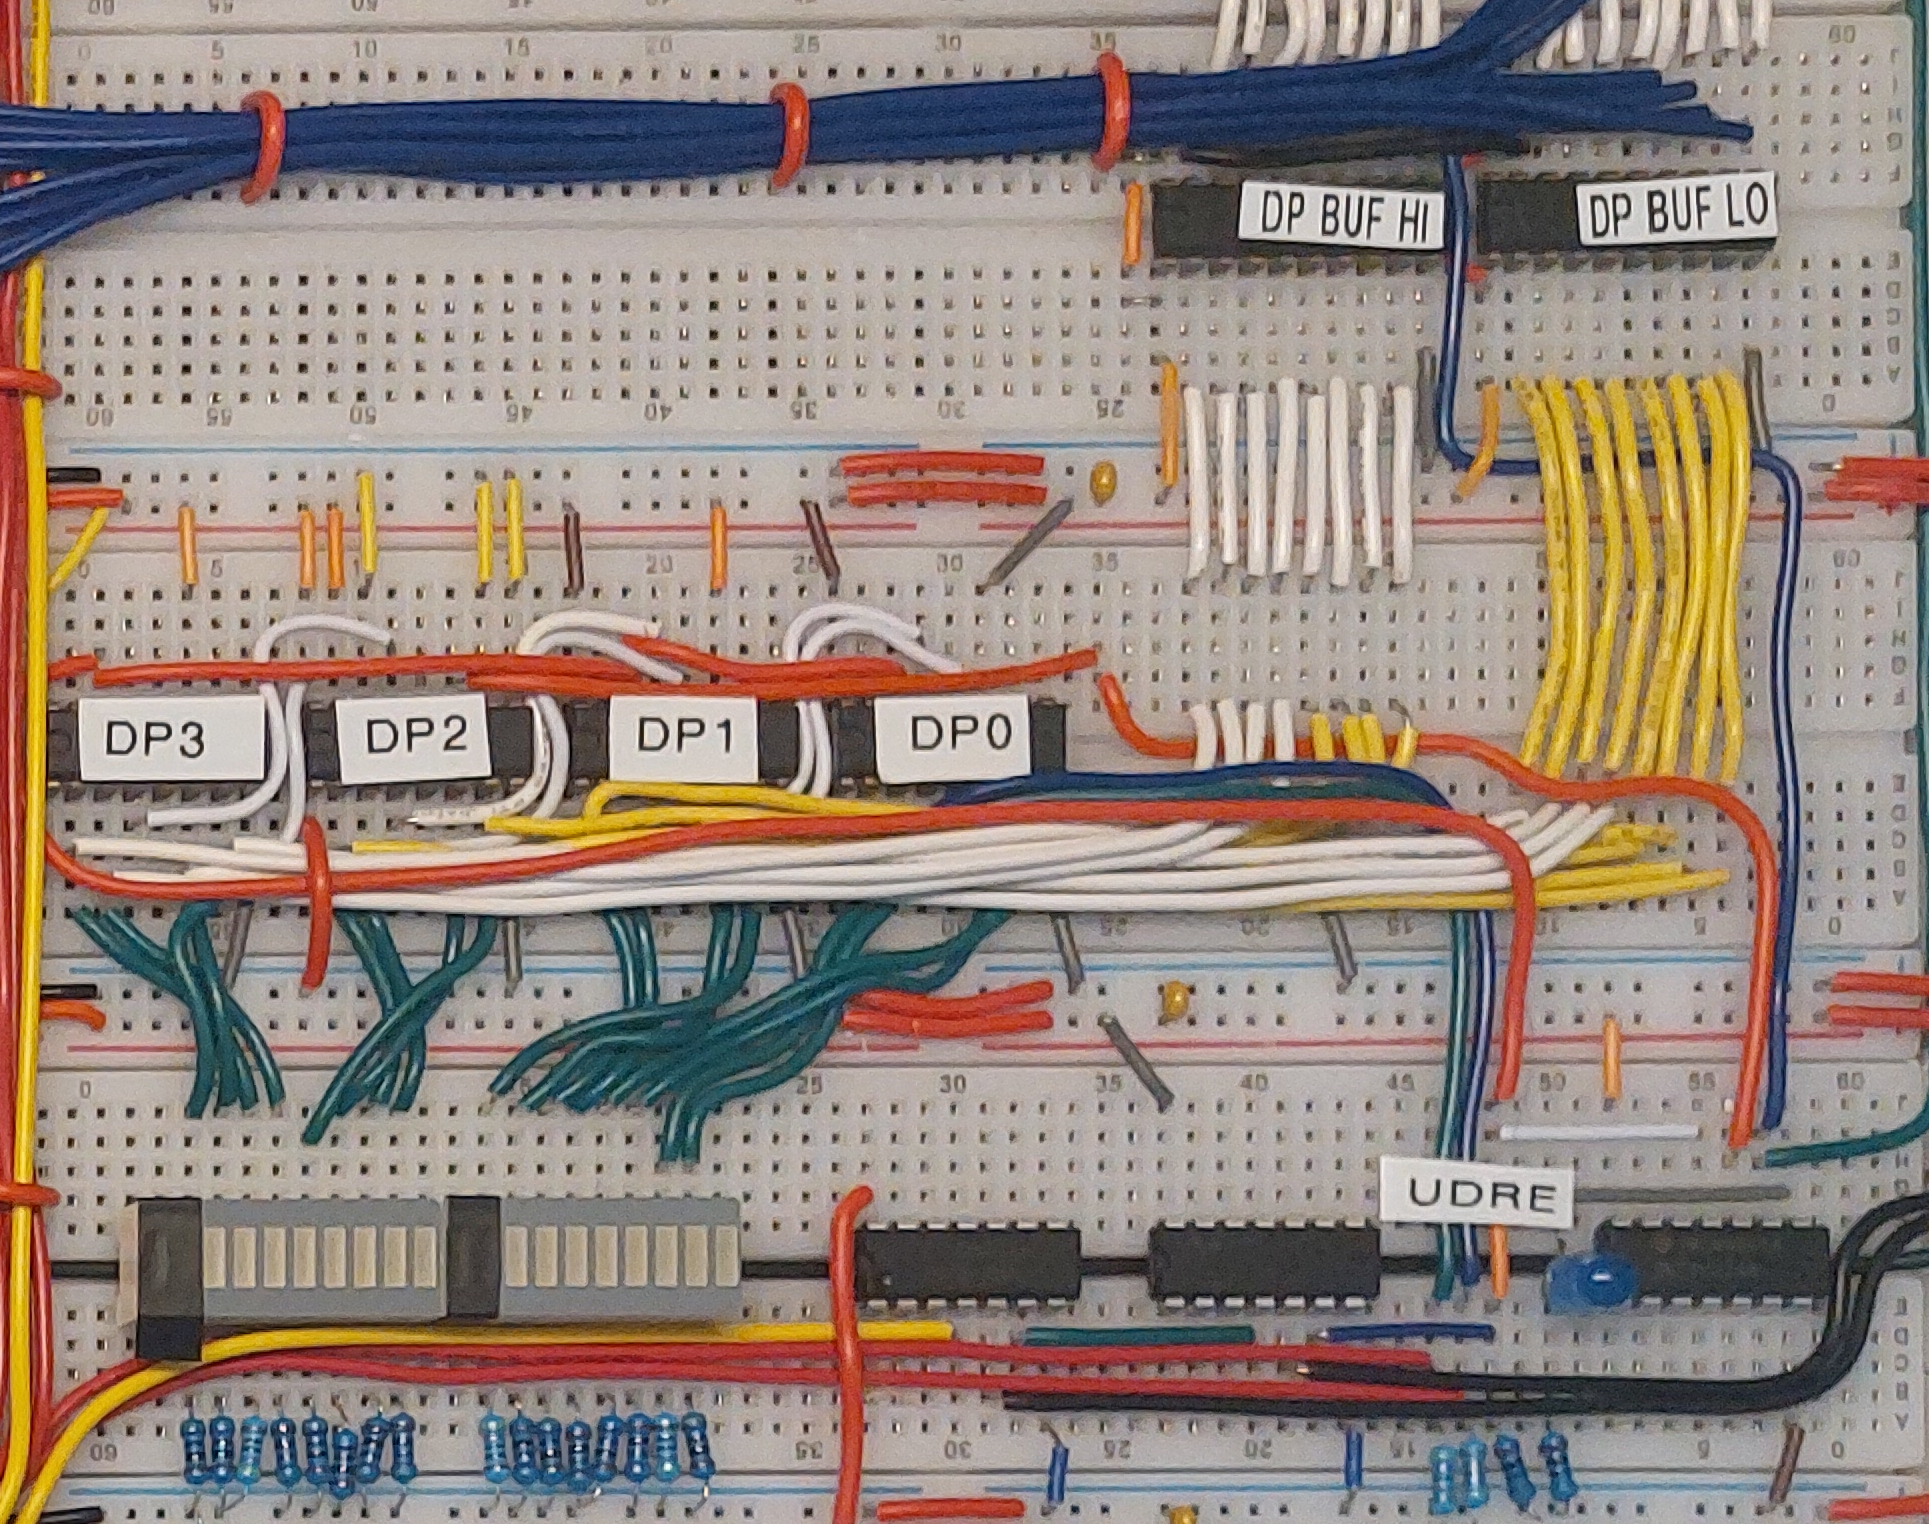
\includegraphics[width=0.6\textwidth]{img/dpregistercloseup}
  \caption{Close up of the Data Pointer Register Module.}
  \label{fig:dpregcloseup}
\end{figure}

The datapointer register contains the address of the cell currently being operated on. It is a 16 bit value kept in four 74LS193 IC's because of the requirement that is should be able to be incremented and decremented. Their outputs are connected to the address bus through a pair of tristate buffers to prevent bus contention with the stack pointer. Because the first 256 bytes are reserved as the stack (where instruction pointer values can be stored to implement loops), the reset value of this register should be set to 0x0100. This is achieved by resetting all IC's except for the one containing the 3rd nibble, which is reset to one by hardcoding 0x1 to its inputs and connecting the reset line (through an inverter) to the load-pin instead (and clock for synchronization).

This register is special in the sense that it is the only register that should be able to be reset at runtime and without resetting any of the other modules (through the DPR signal). This allows it to be reset to its starting value after initializing the computer when power is first applied (see also Sections \ref{sec:sequences:init} and \ref{sec:sequences:home}). The RESET signal is therefor fed into an OR gate together with the DPR signal before going to the reset pins of the IC's.

Perhaps somewhat confusingly, the schematic (see next page) shows that the SP\_EN signal is used to enable the buffers. Since the bus is shared only between the stack pointer and data pointer, the same signal can be used to enable and disable their respective buffers: when the stack pointer is enabled, the data pointer should be disabled and vice versa. Since the output enable pin of the 74LS245 is active low, the SP\_EN can be fed directly into it. On the side of the stack pointer, the same signal goes through an inverter before going into the buffer. By default, when the stack pointer is not enabled, the datapointer will provide the address to the RAM. The RAM address input lines will never be floating which means that the contents of the current memory cell (in RAM) will always be visible in the computer.


\subsubsection{Schematic}
A full schematic is provided on the next page.
\includepdf[landscape=true]{schematics/datapointerregister.pdf}


%%%%%%% DATA REGISTER

\subsection{D Register Module}
\begin{figure}[H]
  % TODO: add annotations to the image
  \centering
  \includegraphics[width=0.6\textwidth]{img/dregistercloseup}
  \caption{Close up of the Data Register Module.}
  \label{fig:dregcloseup}
\end{figure}

The data register holds (a copy of) the value in memory currently pointed to by the datapointer. In the computer, it is located in the top left corner. It is based around the 74LS193 counting register and driven by the register driver described in Section \ref{sec:implementation:registerdriver}. The output is buffered in a tristate buffer (74LS245) before being connected to the databus. A second buffer is used to send all zeroes to the high byte of the databus since the data is only 8 bits wide. The buffers are set to output-mode only (even though the register is able to read from the bus as well) because the 74LS193 chips have seperate pins for incoming and outgoing data. The incoming data is read from the bus directly without going through a buffer.

This module also produces the Z flag, indicating that it is currently containing the value 0. This is achieved by sending the output through an array of OR gates and finally an inverter. The output is then sent to the second half of the instruction register which is responsible for keeping track of the flags.

Because the 74LS193 is loading asynchronously, the clock is gated together with the LD\_D signal through a NAND gate in order to load synchronously with the clock when the LD\_D signal is high (the load-pin on the '193 is active low). The necessity of a NAND gate meant it was easier to also implement any inverters needed in the circuit in terms of NAND gates.


\subsubsection{Schematic}
A full schematic is provided on the next page.
\includepdf[landscape=true]{schematics/dataregister.pdf}

%%%%%%% INSTRUCTION POINTER REGISTER

\subsection{IP Register Module}
\begin{figure}[H]
  \centering
  \includegraphics[width=0.6\textwidth]{img/ipregistercloseup}
  \caption{Close up of the Instruction Register Module.}
  \label{fig:iregcloseup}
\end{figure}

The instruction pointer register holds a 16-bit value representing the address of an instruction in program-memory, stored in an EEPROM module (see \ref{sec:implementation:sigfetch}). Because the size of the available address space is $2^{14}$ instructions, the final two bits of the IP are not used. Red LEDs have been connected to these bits to quickly identify programs that try to address this non-existing part of program memory. The register IC's (74LS193) are driven by the register driver.

The IP is connected to the databus through two tristate buffers (74LS245) to avoid bus contention with the datapointer and keyboard module. It needs to be connected to this bus in order to write its value to the stack when a loop is entered. When exiting from a loop, a value is read back into the register through a direct connection to this bus (without going through a buffer). Because loading is done asynchronously on the '193, the load signal is NAND'ed with the clock to make loading synchronous again.

\subsubsection{Schematic}
A full schematic is provided on the next page.
\includepdf[landscape=true]{schematics/instructionpointerregister.pdf}

%%%%%%% STACK POINTER REGISTER

\subsection{SP Register Module}
\begin{figure}[H]
  \centering
  \includegraphics[width=0.6\textwidth]{img/spregistercloseup}
  \caption{Close up of the Stack Pointer Register Module.}
  \label{fig:spregcloseup}
\end{figure}

The stack pointer is an 8 bit value representing a memory address in the range 0x00 - 0xff, which has been reserved to hold instruction pointer values. This is necessary for implementing conditional loops. When a loop is entered, the current value in the IP register is stored on the stack at the address pointed to by the stack pointer. The SP module is therefore connected to the same RAM address bus as the datapointer, which means it should go through a tristate buffer to avoid bus contention.


\subsubsection{Schematic}
A full schematic is provided on the next page.
\includepdf[landscape=true]{schematics/stackpointerregister.pdf}


%%%%%%% LS Register

\subsection{LS Register Module}
\begin{figure}[H]
  \centering
  \includegraphics[width=0.3\textwidth]{img/lsregistercloseup}
  \caption{Close up of the Loop Skip Register Module.}
  \label{fig:spregcloseup}
\end{figure}

The Loop Skip Register (LS) is used to provide the skip flag (S, see \ref{sec:architecture:ls}). It is implemented using two 74LS193 binary counters and is connected to the decoders of the Register Driver in order to be able to be selected by the control logic. The S flag is compiled from both register IC's by sending all 8 output-bits to an array of OR-gates; when any of these bits are high, the S flag will be asserted, indicating that the computer is in the process of skipping the current loop.


\subsubsection{Schematic}
A full schematic is provided on the next page.
\includepdf[landscape=true]{schematics/loopskipregister.pdf}



%%%%%%% RAM Module

\subsection{RAM Module}
\begin{figure}[H]
  \centering
  \includegraphics[width=0.6\textwidth]{img/ramcloseup}
  \caption{Close up of the RAM Module.}
  \label{fig:ramcloseup}
\end{figure}

\subsubsection{SRAM}
The RAM module is mainly used to store the 8-bit data of the BF memory-tape. However its secondary purpose is to also store the instruction-pointer values when loops are handled, which are 16-bit in size. Therefore the RAM module contains two 512K x 8-bit SRAM chips (AS6C4008) for a total of 512K 16-bit memory-cells. The second chip is therefor only used to store the high-byte of the IP's stored on the stack (at most 256 values). The remainder of the capacity of this chip is not used at all, since the datavalues are only 8 bits in size.

\subsubsection{Buffering}
The AS6C4008 already provides a Chip Enable input which is supposed to be used when the data is connected to a databus. When this input is inactive, its outputs are in a high impedance state to avoid bus contention with other devices. However, in this project we need the data currently pointed to to be visible on an array of LED's, which means that the chip should be enabled basically at all times (except when writing to it). Additional logic is used in conjunction with a pair of 74LS245 tristate buffers to intercept the outputs before making them available on the bus through the buffers. The truthtable for this logic is incorporated in the schematics below. The LED's are not shown in the schematic, but can be connected directly to the datalines of the RAM in this configuration. 

\subsubsection{Schematic}
A full schematic is provided on the next page.
\includepdf[landscape=true]{schematics/rammodule.pdf}


%%%%%%% CONTROL UNIT

\subsection{Control Unit}\label{sec:implementation:cu}
\begin{figure}[H]
  \centering
  \includegraphics[width=0.6\textwidth]{img/controlunitcloseup}
  \caption{Close up of the Control Unit.}
  \label{fig:controlunitcloseup}
\end{figure}


\subsubsection{Partitioning}
The control unit is responsible for sending the appropriate signals to each of the modules. The general idea is that the current instruction pointed to by the IP (4 bits) together with the state flags (another 4 bits: A, V, S and Z) and the cycle count (3 bits) combine together to form an (11 bit) address into a set of three EEPROM chips (AT28C64B), each of which contains part the signal configuration corresponding to that combination of state and instruction. When clocked by the decoder-clock (D\_CLK), the values currently at this address are loaded into the registers (74LS173) and asserted onto their respective modules, which will act upon them on the next pulse of the M\_CLK signal.

Based on the physical layout of the board, the following configuration was used to construct an address into the EEPROMs.
\\
\begin{center}
\begin{tabular}{r|ll} 
  Address Bits & \\ \hline
  0-2  & Cycle count & ($000_2$ - $111_2$) \\
  3-7  & Instruction & ($0000_2$ - $1111_2$) \\
  8-11 & Flags & ($0000_2$ - $1111_2$) \\
  12-13 & Unused & 
\end{tabular}
\end{center}

The three EEPROM's have been programmed using a custom built EEPROM programmer based around an Arduino Nano, combined with a python script (\texttt{bflash}) that is able to send a binary image to the Nano over a serial connection. The images that store the microcode tables have been generated by Mugen (see \ref{sec:utilities:mugen}), a utility developed to make the microcode programming more maintainable. Mugen generates the images from a specification file. The relevant part of the specification for the BFCPU is shown in the listing below and is a direct representation of the microcode shown in Table \ref{tab:microcode}.

\lstinputlisting[firstline=53, firstnumber=1]{../src/microcode/bfcpu.mu}


\subsubsection{Program ROM}
The actual BF program is stored in another 8K EEPROM chip (AT28C64) and is addressed by the instruction pointer as mentioned before. Since each BF instruction only needs 4 bits to be encoded (there are less than 16 different instructions), we can store up to 16K instruction in the chip by packing 2 consecutive instructions together in a single byte (handled by the assembler). Rather than using bit 0 from the IP directly as address bit 0 on the EEPROM, it is used as the data-select signal to a 74LS157 multiplexer. This multiplexer takes 1 select-bit and two sets of 4 databits. Depending on the value of the select-bit, one of the sets of 4-bit data is sent to its outputs. This allowes us to select either the low or high nibble of the data in the EEPROM, effectively doubling the amount of instructions that can be stored and retrieved.
 
\subsubsection{Cycle Counter}
The cycle counter is another 74LS161 that simply counts up and sends its outputs (bits 0-2) to address lines 0-2 of the microcode EEPROM chips. It is reset when it receives the CR signal (which becomes active when an instruction has completed).


\subsubsection{Schematic}
A full schematic is provided on the next page.
\includepdf[landscape=true]{schematics/controlunit.pdf}

%%%%%%% IO Module
\subsection{IO Module}
The IO system is handled by an ATMEGA328P microprocessor, commonly found in the Arduino Uno. It has three main functions:
\begin{enumerate}
\item Drive the screen and display contents from the bus when instructed to by the \texttt{EN\_OUT} signal.
\item Handle keyboard input and provide input data to the bus when instructed to by the \texttt{EN\_IN} signal.
\item Supply a menu system to alter its settings using two buttons.
\end{enumerate}

\subsubsection{Buttons and Menu}
Two buttons are provided to interact with this system. They are mainly used to scroll the screen but can also be used to access and navigate a menu (Figure \ref{fig:menuscreen}). This menu let's the user do the following:
\begin{enumerate}
\item Clear the screen and keyboard buffer.
\item Change the display-mode. By default, incoming data is interpreted as ASCII characters. When it should be displayed as raw numerical values (either in base 10 or 16), this option can be selected from the menu. When in either of these numerical modes, a delimiter character can be selected to separate bytes visually.
\item Set autoscrolling on/off. By default the screen will scroll its contents when they overflow to always keep the most recent data in view. When new data is displayed, the screen is always scrolled to display this data. Setting autoscroll to `off' will disable these features.
\item Echo on/off. When running an interactive program that requires keyboard input, the user probably wants to see what is being typed. This is the default behavior (echo on). If for some reason the keypresses should not be displayed, this option can be disabled.
\item Reset to default settings. Whenever settings have been changed, the new settings will be saved to the persistent EEPROM memory of the MCU and loaded back on startup to make the settings persist when the MCU is powered down. This option allows you to revert all changes and load the default settings back in.
\end{enumerate}

\begin{figure}[h]
  \centering
  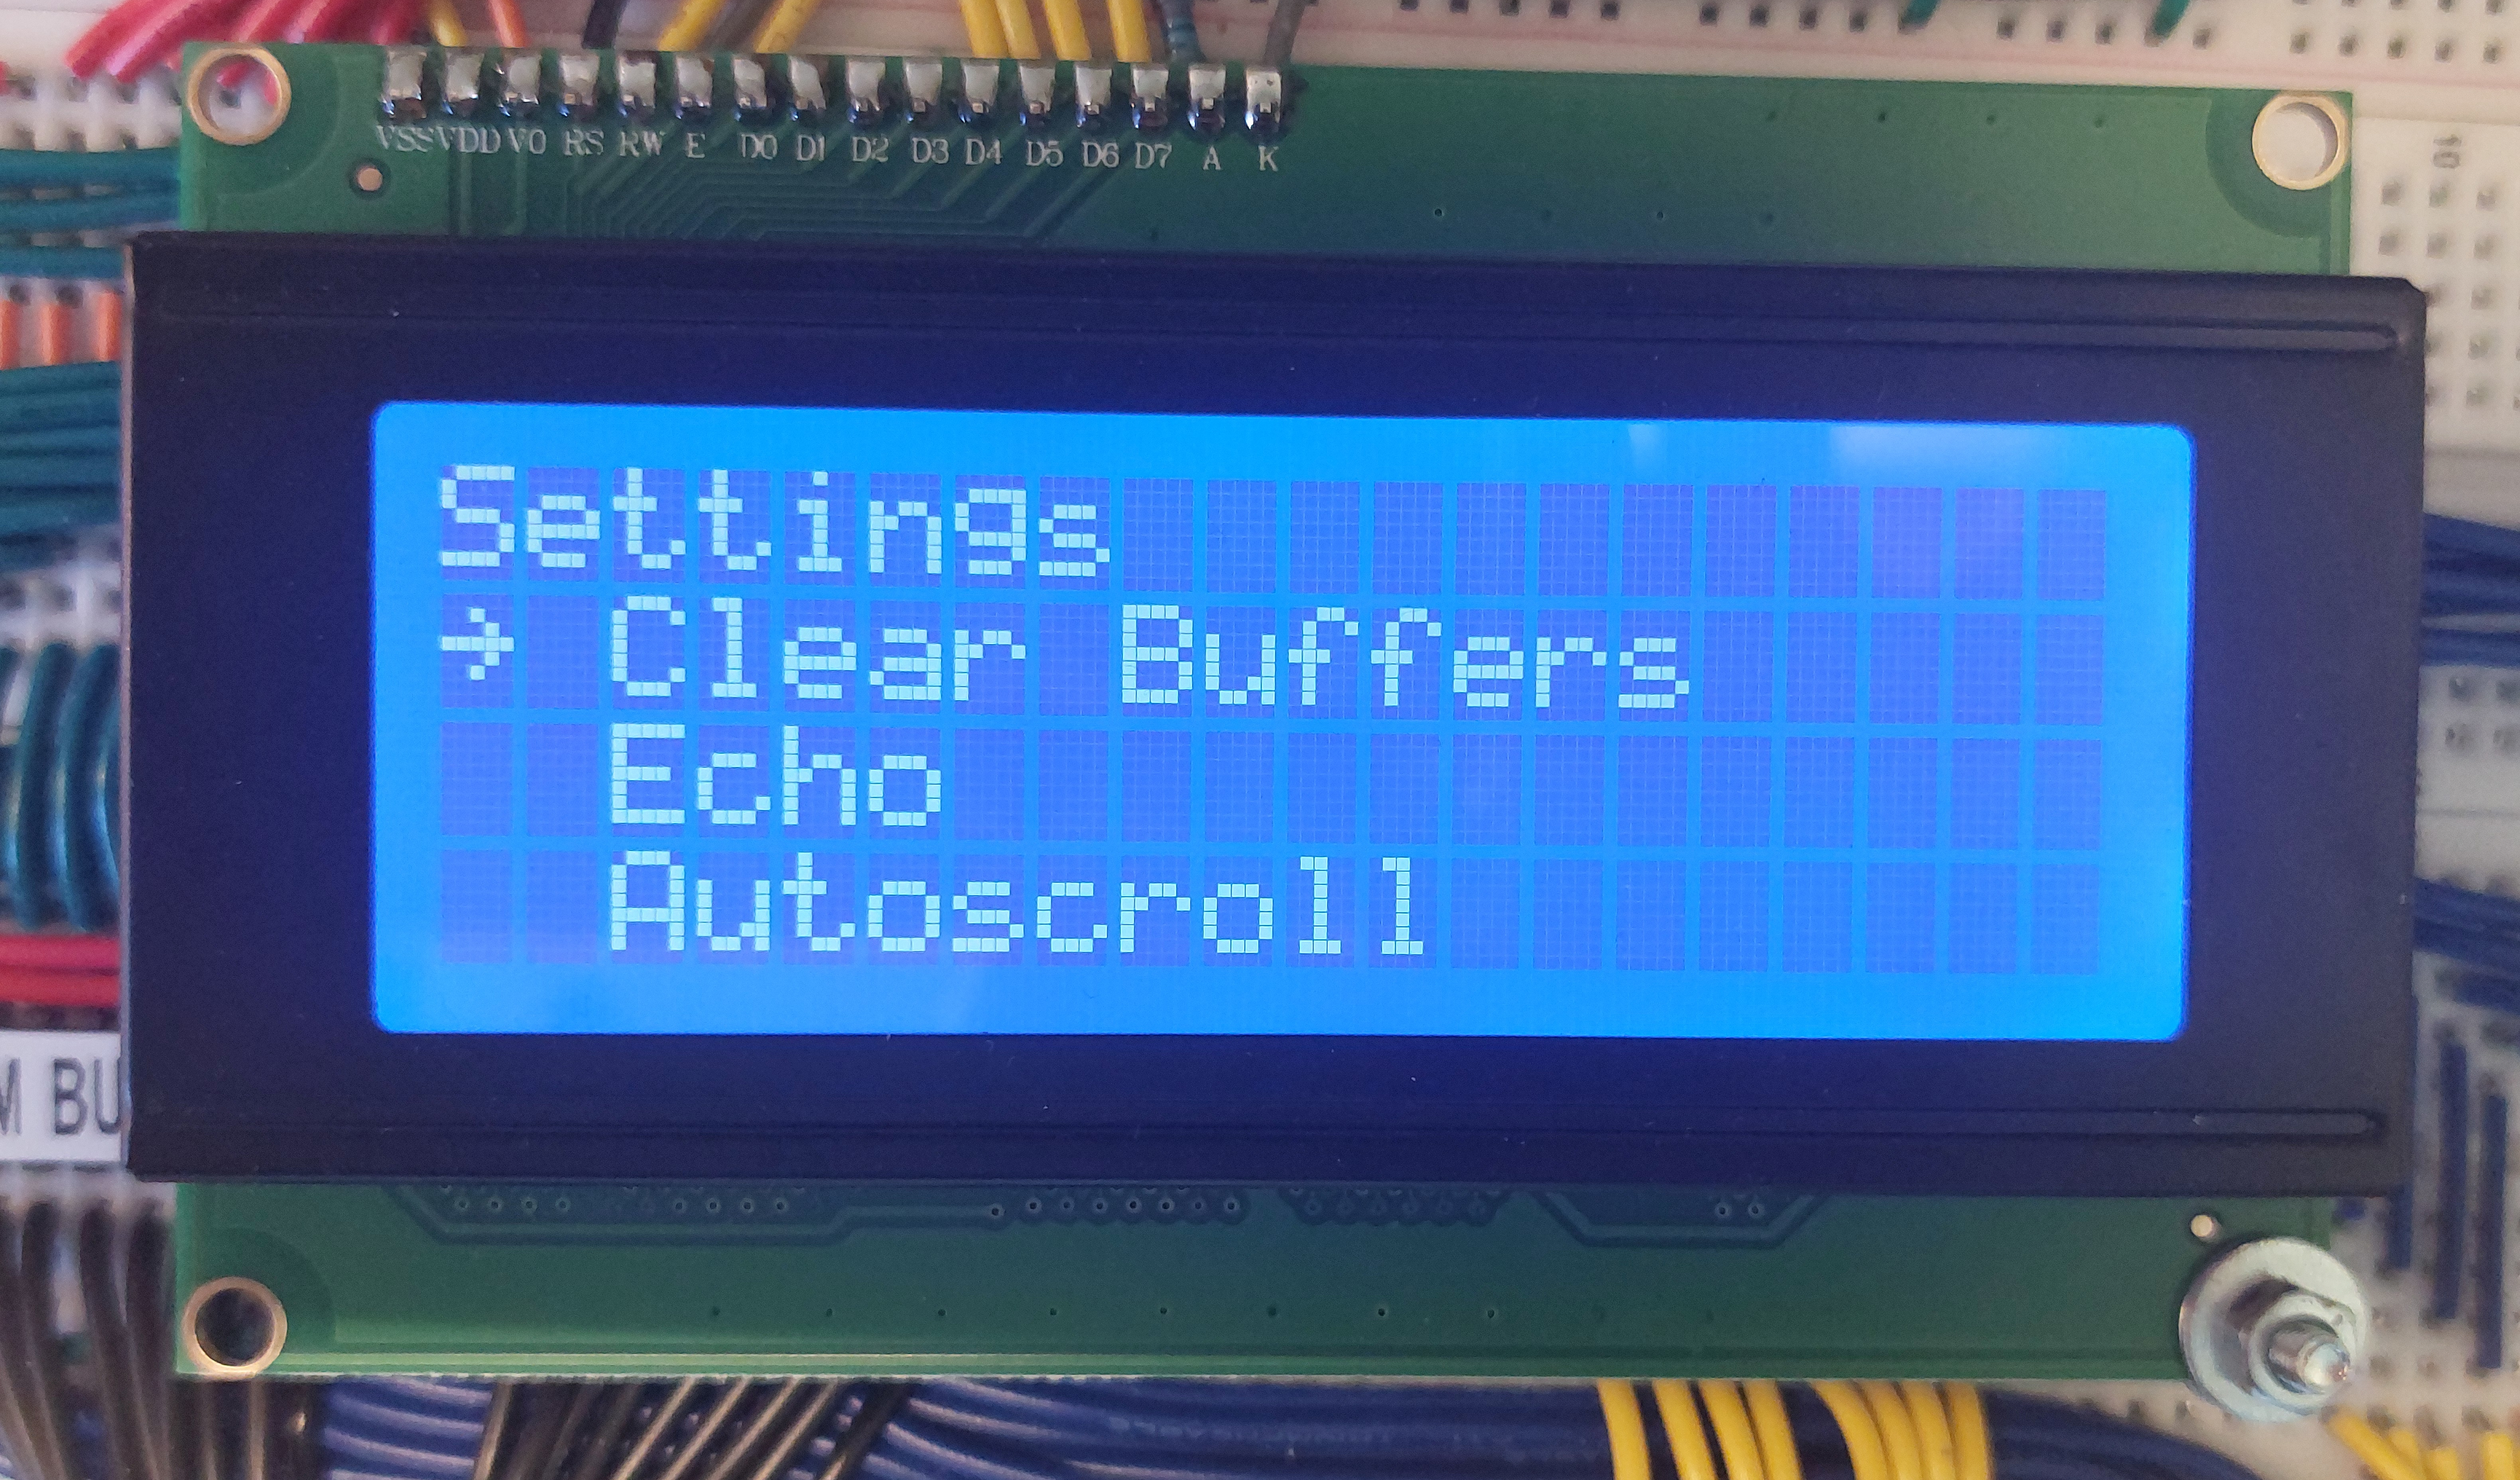
\includegraphics[width=0.5\textwidth]{img/menuscreen}
  \caption{Part of the menu that is accessible by pressing both scroll-buttons simultaneously.}
  \label{fig:menuscreen}
\end{figure}


\subsubsection{Handling Input and Output}
\paragraph{Output} The \texttt{M\_CLK} signal is connected to an interrupt pin of the MCU. On every interrupt triggered by the clock, the MCU will check the status of the pin connected to the \texttt{EN\_OUT} signal. When it is high, all of the pins connected to the databus are read to reconstruct the byte present on the bus. This value is then displayed on the LCD. Listing \ref{lst:io_isr} shows the code for the interrupt routine running on the MCU.

\paragraph{Input} Handling input from the keyboard is slightly more involved. When interrupted by the clock, if the \texttt{EN\_IN} signal is found to be high, the MCU goes into a 3-clock-cycle routine. During the first cycle (when the \texttt{EN\_IN} signal went high), the IO pins are set to output-mode, data is fetched from the keyboard and put on the bus. On the second cycle, it does nothing at all; this is when the computer reads the value into the D register. Then on the 3rd cycle, when the computer should have completed reading the value into its register, the pins can be reset to input-mode (high Z) and the MCU will wait for its next instruction. The flow of the state-machine that implements this algorithm is shown in Figure \ref{fig:isrflow}.

\begin{figure}[H]
  \centering
  \includegraphics[width=\textwidth]{img/isrflow}
  \caption{Control flow inside the ISR running on the microcontroller.}
  \label{fig:isrflow}
\end{figure}

\subsubsection{Shift Register}
To decrease the number of pins needed to drive the LCD module, a shift register is used. In the current implementation, every pin except the RX/TX pins (reseverd for debugging over a serial connection) is used so using the shift register (74HC595) was vital.

\subsubsection{LCD Screen}
The software was written in such a way that most common LCD character screens (compatible with Hitachi the HD44780 driver) will be handled appropriately. Both a 16x2 and 20x4 have successfully been installed in the computer. A modified version of the \texttt{LiquidCrystal\_74HC595} library was used to implement the LCD driver.

\subsubsection{Keyboard}
The IO module can only handle input from PS/2 compatible keyboards. A modified version of the \texttt{PS2Keyboard} library was used to implement the keyboard driver.

\subsubsection{Software}
The full source code for the IO module can be found on Github: \url{https://github.com/jorenheit/bfcpu/tree/main/src/io_module}.

\subsubsection{Schematic}
A full schematic is provided on the next page.
\includepdf[landscape=true]{schematics/iomodule.pdf}
